\documentclass[12pt]{report}

\usepackage[margin=1.0in]{geometry}

\usepackage{graphicx}
\graphicspath{{./images/}}

\usepackage[
backend=biber,
style=numeric,
sorting=none
]{biblatex}
\addbibresource{references.bib}



% Title Page
\title{Robinson Observatory Telescope Refresh}
\author{Bradley Glaser, Derek McCrae, Bryan Ocbina, Justin Rudisal}


\begin{document}

\maketitle

\begin{abstract}
\end{abstract}

\section*{Executive Summary}
Do what you say you will do.\cite{heinrich}

\section*{Technical Content}

\subsection*{Project Narrative}

The Robinson Observatory is a facility at UCF that is used for both education and research on the topics of astronomy.  It is run by members of the Planetary Sciences Group and the Astronomy Society in the physics department.  The observatory provides high resolutions of astronomical objects and various events and programs involving the UCF and Central Florida to connect members of the community to astronomy .  The main telescope at the observatory is a 20-inch f/8.2 RCOS Ritchey-Chretien telescope and has recently had issues regarding its mobility.  The telescope is able to align itself to a starting reference point, but when given instructions to move to a certain coordinate, the telescope will unreliably move towards the coordinate without any relation to its physical capabilities or location.  This leads to a layer of issues.  The main issue involves being completely off-course of the desired coordinate.  The telescope software will either output warnings too early or too late and not prevent the telescope from colliding with its mount which causes damage to the entire system.  This is a hazard to the staff and the powerful and high cost telescope itself.

The origin of the problem is questioned whether it is a mechanical issue or a problem with the various software that are involved in operating the telescope.  Our computer science team alongside the electrical engineering and mechanical engineering teams will work together to determine the issues and provide solutions that will assist in leading bringing back the telescope to full functionality.  The main concern of the team at the observatory in regards to computer science is that the software of all of the components of the telescope are able to communicate properly on Windows 10.  The components are the telescope, TheSkyX Professional software, the focuser software, and the dome control software.  Meeting this specification will require research into each component of the system and also research into possible software/driver compatibility issues.  The knowledge to code drivers ourselves may be required.  Possible roadblocks may be that certain softwares are not updated or maintained to current standards which would require an overhaul of the system to have all components compatible.  Having the telescope and its surrounding system compatible will be the main objective of our project.

The second objective for our team will be to assist the research opportunities  and community outreach events available at the Robinson Observatory.  Our team will be designing a database capable of storing the images, and their metadata, taken directly by the telescope.  This database will function alongside a user-friendly website that can be used by the community for sharing images and also by the astronomer team to conduct research.  The images will be indexed with their relevant data and a search functionality will be available.  This will provide storage for the data collected at the observatory and assist in long-term research.  On the community side, the website will allow the observatory to easily share images with those interested.  A possible stretch goal is to use machine learning to search images for known objects based on a gathering of previous tagged images of the object.

The third objective will be to assist the electrical engineering team in modeling the black box which serves as the main component for issuing commands to the telescope.  The model will replicate the functionality of the telescope in turns of movement and sending and receiving data.  The current goal for the model is to be able to track the sun or moon within the accuracy of a degree.  This model will assist future teams as the complexity of the black box has been deemed to be too large in scope for a single year senior design team.  The reverse engineering of the black box will be useful for moving away from proprietary systems and give greater control to the team at the observatory in terms of what they would like out of the telescope, making it more programmable to their personal needs.

There are also a series of additional objectives pertaining to recording and storing astronomical data that will be obtained from the software when taking images.  They are outlined in the later sections of this document but serve to either allow for better research opportunities for the astronomer team or to simplify a process and improve the functionality of the facility through accessibility between systems at the observatory or allowing for online access to the faculty or community.

The refresh of the Robinson Observatory is a goal that is extremely important to each member of our team.  This project serves as an opportunity to give back to our university for all the experiences we have gained in our past few years here.  A reminder of all the knowledge we have accumulated into a single project demonstrating our technical skills and problem solving ability.  We hope to be able to remember our senior design project proudly as we bring an end to our time with education and proceed into the professional world of computer science.  Each of our members would also like to address their own personal interests and motivations in this project.

\subsection*{Personal Interest}

\subsubsection*{Justin Rudisal}

My personal interest in this project is twofold with the first part being due to the subject area being space, and the second due to the project area involving a level of mechanical integration. Within my own personal experience with Internships, I have worked heavily with website development and database management. However, I have absolutely no knowledge of mechanical systems and how a computer communicates with a physical, moving part. My dream goal is working in the creative entertainment programming field, such as Universal Creative or Disney Imagineering, and so I need this basic machine programming experience to be successful in my pursuit of a career in those areas.

I also have been in love with space and space exploration for as long as I can remember, and so much so that I originally was planning on doing a double major in both Computer Science and Astronomy until I sadly realized I could not afford to pursue both. So when I heard of the senior design project that would be combining both the area of knowledge that I wish to learn more in with an area of passion that I love, I knew I had to jump on it as quickly as I could.

Other major considerations of mine for this project include the fact that it is a completely open-source undertaking. The end goal of this is to be able to document and demonstrate everything we do so that other small observatories around the world can easily duplicate our results. Projects such as that are the ones that drive my passion in programming, as well as the engineering field in general, because I fully stand behind and support anything with altruistic goals that benefits other people for the common good. I personally believe intellectual progress is achieved from the sharing of knowledge freely, and not from the selling of it for a profit.

I also want to leave a legacy behind me within my university that I have called home for the past handful of years, and that has brought so many different opportunities into my life. I want to give back to the place that has given so much to me. Being able to refresh the telescope and have my name on such a substantial undertaking is one way that I can give back and leave that legacy. I can come back years later, point at the observatory, and say "I helped repair that and bring it into the modern era". Now that is both a great resume builder, and overall achievement to be proud to talk to others about.

I remember one of my most favorite experiences from my first years at college was actually going to the observatory for "Knights Under the Stars" throughout my first few semesters, and being able to watch the telescope work and see the screen show images of our galaxy. I thought that was one of the most fascinating things ever, and it sparked an even bigger passion in astronomy in my life. Lack of time, and it's breaking, caused me to stop going as I got into my higher level classes, but that initial impression left on me caused me to instantly want to help repair the observatory when it was announced as a senior design project.

\subsubsection*{Derek McCrae}

I want to embark on this project primarily for my interest in space. Growing up near the Kennedy Space Center, I was viewing the shuttle launches from a young age and dreamed upon what is out there. A sight I will always want to see firsthand has been strengthened by the pictures provided by telescopes. Telescopes provide a great photos of our universe that can't be currently reached by humans like the Hubble Telescope showcasing the Pillars of Creation or a simple home telescope to view Jupiter. This passion that has grown stronger with the advancements being made for commercial trips to space, especially the advancements by SpaceX. The technological advancements SpaceX has made with getting their boosters to land safely back at a landing pad simultaneously is one of the coolest things I have seen in the last decade. SpaceX along with Virgin Galactic have brought excitement back to space exploration. Some great memories I have include watch parties that had telescope viewings of either a launch, or eclipse, or viewing of another planet.

I had two events that greatly enhanced my passion for space. The first one happened when I was in 7th grade and our class trip was to the Kennedy Space Center. We were able to tour the facilities and sleep under one of the rockets that had on display. The trip helped gain new knowledge and greater appreciation of space. The second event happened freshman summer of high school on a trip to North Carolina. I was family on the side of a mountain in some cabins. One night the mountain staff held a viewing party. My family along with other guests were able to view the stars and use a telescope to see planets only viewable at that time of the year. The event showed me how the topic of space can bring people together.

These two events are a cornerstone to why I wanted to be apart of this project. I know firsthand how viewing parties can bring people together and the knowledge can be beneficial. Not many people own their own personal telescope so this observatory can give those interested a better way to view the sky. To know, I will have a helping hand in allowing activities to once again be performed at the observatory is exciting. The observatory can bring back “Knights Under the Stars” allowing many the current unavailable opportunity of getting to see the stars up close. The observatory could even provide new research study opportunities for those at UCF.

The next reason I chose this project was to build experiences on ideas I have yet to work with. My initial interpretation for this project was a new software needs to be created to help the telescope return to working order. I have learned how to code basic programs and taught programming stepping stones over the past few years without getting any real world experience. I have been eager to apply my knowledge to develop something that will be used past my educational career here at UCF. Furthermore, it will be applying this knowledge to help build something in an industry I am passionate about.

My final motivation for this project is the ability to leave behind a legacy. Of course, the legacy could become poor if this project isn’t completed properly but with proper completion, our solution will outlast my time here at UCF. This refresh could impact this university and space exploration for the next few years and that provides a strong legacy.

\subsubsection*{Bradley Glaser}

I have always had a deep love for everything space. Likewise, my science classes were always some of my favorite courses in school. From a very young age I was always asking questions and some of the biggest unanswered questions are extraterrestrial. The exploration and study of the cosmos must be one of humanity’s priorities if we are to advance as a civilization. I realize that my contributions to the Robinson Observatory are not quite earth shattering. However, I am happy to be able to say that I am a small part of that undertaking.

My father was always a very strong influencer in my life and he has always pushed me to pursue my goals. When I was in elementary, he got me my first childhood telescope. It was one of my most prized possessions. I kept it for many years and I have fond memories of stargazing with my friends and family. This project is an amazing opportunity to work on a full size telescope. One the day that we were assigned the projects, I called my father and told him about my selection. He was over the moon about it. I cannot wait to dig into this project and make it a reality.

My fiance and I have a special connection because of stargazing. When we lived in Utah, some of our earliest dates were spent on the top of a mountain looking at the stars and moon. We would hike up the mountain as the sun went down and then spend our time laying on the ground and watching for shooting stars. Our relationship was built on a shared love of science and space. Space has been a big influence on my life and I hope that my involvement in this project will help others to capture that same magic.

Intellectual property is a big concern of mine. I understand the value of having outside companies come to UCF and pitch projects. Students need real work experience and those businesses are able to provide it. However, the cynical side of me sees these businesses profiting off of the work senior design students are performing for them. Thus, I wanted to choose a project that would be internal to UCF. That way I can be sure that my time spent will not just be putting money into someone else’s coffers.

I wanted to work on a project that was tangible. Many of the projects presented for us to pick from were either esoteric or difficult to explain to non technical persons. Explaining that I will be on the team that fixes UCF’s observatory is immediately easy for anyone to understand. Likewise, I felt that potential employers would be more responsive to a project which was for the immediate betterment of others. It is hard for the average person to understand how “analyzing blockchain correctness” will affect them. However, I am able to point to the telescope and say “you couldn’t visit that before and now it works”. That direct impact is something that I wanted to have for a project.

Being able to contribute to UCF and help future students foster their love of astronomy is a dream come true. I hope that my contributions to this project will help others discover their passions. Similarly, the ability to leave a legacy behind at UCF is a big bonus. Many of the projects presented to us seemed fleeting or shallow in my opinion. They dealt with trivial things that, in the case of blockchain, might not even be relevant in the coming years. I hope that our contributions are more substantial and that they will stand the test of time.

\subsubsection*{Bryan Ocbina}

After hearing the pitch for this project, I realized being able to provide a meaningful impact on the UCF community was significant for myself.  I have grown up in Orlando all my life and have been ingrained to love all thing related to Florida from Disney and mickey mouse to the beaches and manatees to watching rocket and shuttle launches liftoff from Kennedy Space Center, with pure amazement every single time.  As I enter my final year as a Computer Science student, I would like to create a lifelong experience and memory here in my hometown before I finish my education, graduate, and begin to use my knowledge and technical skills in the professional world wherever my career may take me.  Aiding in the Robinson Observatory refresh is a project that aligns with my interests and goals and is my first choice amongst the about fifty projects presented to us.

One of my favorite memories is going on a camping trip a few summers ago and being to stargaze with close to zero light pollution.  The night sky at this time was and is still the most amazing and unforgettable sight I have ever seen.  I had a realization after seeing the sheer number of stars and the surprising amount of color of how much beauty we miss out on living in the city with lights everywhere.  Likewise, as another unforgettable experience was a viewing of a nighttime shuttle launch from my home in Orlando that lit up the sky as if the sun was rising.  Space and the stars above bring out childlike wonder in myself and brings excitement as our team begins to develop our design for the Robinson Observatory refresh.  To be able to once again share images from the telescope at the observatory and hopefully inspire some childlike wonder in someone else is an important part of this undertaking.

The UCF community and Central Florida as a whole is a wonderful center for growth and dreams.  Community outreach is a valuable aspect of this project.  Public events such as “Knights Under the Stars” held at the Robinson Observatory allow for people of all ages to explore the night sky and learn about our solar system and various nearby stars or other celestial phenomenon.  However with the main 20-inch telescope out of commission, the ability to view the night sky at these events is undoubtedly weakened.  We hope to not only restore this functionality but to also add on and allow for images from the 20-inch telescope to be shared more easily with the community.

As another part of community outreach, a decisive part of joining this project includes the open-source aspect of working with UCF.  This project serves to better the research opportunities available locally in Central Florida and our work done with the observatory will not be used to profit some business’s latest product.  The story of the project is much more involved and personal than the other projects pitched to our class.  We are able to not just present a fleshed out, functional telescope as a project we worked on but as an entire experience that could serve to inspire a future astronomer, aerospace engineer, or astronaut.

This project will be my number one priority for my remaining time as a student and I hope to gain as much as I can while working with everyone at the observatory and the other student teams as we share our experiences of our different fields and do our best to create an unforgettable experience.  Altogether, the Robinson Observatory refresh project serves as a platform to express my sincere appreciation for my hometown Orlando, Florida. I have many hopes for my senior design team that we will be able to accomplish some amazing features that will modernize the observatory and that will be used and remembered for many years after we have all graduated.  To be able to come back home, visit the observatory, and tell others that I worked on this feature or component at the Robinson Observatory would be a wondrous feeling.

\subsection*{Broader Impacts}

Getting the telescope and observatory working will help with both the different organizations that contract out the observatory for their own scientific pursuits, as well as enhancing its ability to reach out to students and the surrounding community with an accessible means to the stars. Even those who are not local will be able to benefit from this project due to one of our goals being to create an online public viewing platform for what the observatory is currently observing and completing. This opens it up to anyone with access to an online device to actively engage with the observatory, as well as the scientific space community at large. Our goal is to create both an online portal for the observatories sponsors to access the device, as well as crafting a learning environment for everyone.

This online outreach will also help spearhead engagement within space exploration and space overall within STEM groups both in the university as well as local elementary, middle, and high schools. Teachers will be able to pull up the current observatory pictures and developments, and will also be able to speak on weekly events that the observatory will be hosting. The overall goal is to both repair the observatory and bring it up to operating standards, as well as revamping its public outreach through new websites.

The organization that runs the observatory, Florida Space Institute, is a research group that is funded completely off of scientific grants and personal donations. By repairing this observatory for the Florida Space Institute we are helping an organization that may otherwise have a tough time affording the hiring of professionals to accomplish the intended goals. We are also helping to free up the time of those within the organization who may have had to spend their own time figuring out complicated temporary workarounds for the observatories problems instead of doing the scientific work that they want to accomplish.

\section*{Archive Frontend}

The data gathered by the telescope will need to be accessible by future researchers. Likewise, it might be possible to allow the general public to have access to the data. Either way, the data archive will require a frontend to enable browsing, searching, uploading, downloading, and categorizing the data. The frontend will be a login secured website in order to maximize portability and accessibility. By foregoing a native application, we ensure that the data will be accessible from anywhere with an internet connection. Likewise, we enable the researchers to utilize whatever person computers are most convenient. i.e. laptops, a tablet, an iPad, a cell phone, etc.

Figure \ref{fig:archiveusecase} shows a high level overview of the archive frontend. Each action of the archive system performs modifications in the database when they are accessed by the end-user. The actions will be accessible via the interactive website or via the API directly. This separation of function will enable us to potentially expand our project scope as needed. There may be other applications that can utilize the API as part of our project or future projects.

\begin{figure}[h]
	\centering
	\caption{Archive Frontend Use-Case}
	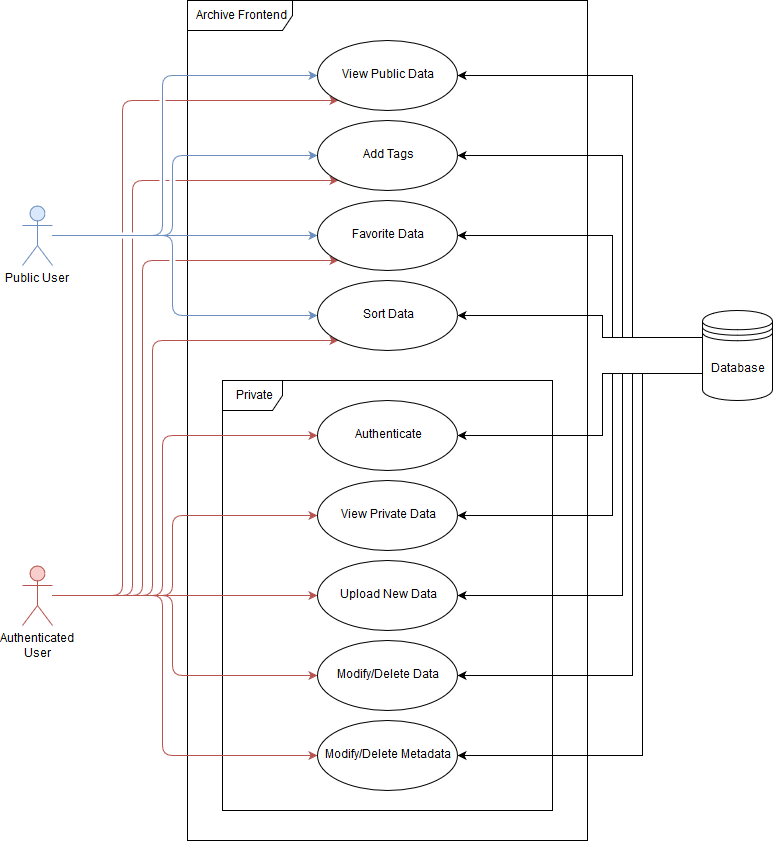
\includegraphics[width=0.75\linewidth]{frontend_use_case}
	\label{fig:archiveusecase}
\end{figure}

The archive will be split into two separate components. Access to the private portion of the website functionality will require logging-in so that the user can be authenticated. Likewise, different users may have access to different sources of private data depending on the security needs of the observatory.

Unauthenticated users will be able to browse the data published as public. We enable said users to perform basic browsing and searching as one would expect. Likewise, we will enable users to add tags and favorites to data. Said information will be stored in the user's cookies until they decide to create an account. Once an account is created, the data stored in their cookies can be uploaded to ensure that the data is persistent across browser sessions.

Authenticated users with the appropriate account permissions will have access to further functionality beyond the basics. They will be able to modify the database directly by uploaded new data and modifying the metadata associated with data that exists withing the archive. Any modifications made by an authenticated user will only apply to data within their permission group. Data may be shared across several permission groups and thus users will only see the modifications made associated with their group. In order to facilitate said functionality, we will need to keep modifications separate from the source data in our backend.

\subsection*{Frontend Frameworks}

Frontend frameworks have become the de facto standard of the web. Industry has moved away from static HTML websites in recent years. Users demand a high degree of interactivity from their websites. Thus, industry has responded by adding more client code in order to facilitate said demand. By utilizing a framework for our project, we will gain vital industry experience that employers are looking for from their applicants.

We opted to utilize a frontend framework in order to facilitate a high degree of interactivity. There are several options for delivering static HTML pages with minimal client-side JavaScript. However, we want to ensure that our client interactions are extremely fast to load. Specifically, sorting data can be offloaded to the client to ensure that one doesn't have to load a new web-page each time that one changes a search parameter. Utilizing a frontend framework enables us to update the data display instantly when said parameters are changed.

There are many modern frontend frameworks which enable developers to quickly create highly interactive websites efficiently. Our frontend solution will need to be data efficient to reduce the strain on potentially poor connections. It is possible that potential users will have a poor internet connection while attempting to access the data. (As is the case in some observatories.) Thus it is necessary to choose the appropriate framework solution which enables rapid development while maintaining a focus on efficiency.

\subsubsection*{Angular}

The Angular web framework was released by Google in September of 2016.\cite{angularrelease} Angular (also known as Angular 2) was released as a replacement for Angular 1. Its release focused on "a wide range of use cases,...[optimization] for developer productivity, small payload size, and performance."\cite{angularrelease} The framework was built from the beginning via "collaboration with the open source development community."\cite{angularrelease} Thus it has received input from many different developers to ensure that it is flexible enough for general use.

Angular utilizes TypeScript as its implementation language which helps reduce bugs associated with loose typing. Typescript also brings many features absent from plain JavaScript which can help to reduce developer time. Utilizing a framework which already utilizes TypeScript will be more advantageous than trying to use it with a framework which was not built to support it.

Angular is built utilizing component objects. The Angular official quick start guide states that "components are the fundamental building blocks of Angular applications."\cite{angularquickstart} These components "display data on the screen, listen for user input, and take action based on that input."\cite{angularquickstart} Components are a good way of breaking one's code up into reusable pieces. By compartmentalizing one's code in this way, there is a reduction in the duplication of effort. Likewise, it creates the opportunity to test each component separately from the rest of the overall application.

Angular is a good candidate for our archive frontend. It was designed to be extremely flexible. Likewise, it is a commonly used industry frontend framework. Employers look for candidates with existing knowledge of frameworks. Thus it would be useful for our team to gain experience using such a common library.

\subsubsection*{Bootstrap}

Bootstrap is an open-source framework originally developed at Twitter in 2010.\cite{bootstrapabout} It was originally a closed-source tool for internal use at Twitter. However, it was eventually open-sourced due to its popularity with the internal Twitter developers. Twitter found that "developers of all skill levels [could jump] in without any external guidance."\cite{bootstrapabout}

Like Angular, Bootstrap also includes components. However, the Bootstrap components are focused on the display of data and abstains from opinions about the structure of one's data. This decoupled nature means that utilizing components ensures that applications built with Bootstrap share a common look and feel. Familiar components ensure that potential users are quick to acclimate.

Unlike other frameworks, Bootstrap relies on jQuery to handle its JavaScript integration.\cite{bootstrapjs} Thus, Bootstrap is much less opinionated on the frontend code structure. This enables developers to create their own code idioms and integrate into existing code bases easily. Likewise, Bootstrap is able to be utilized alongside other frontend frameworks. If we chose to do so, we could utilize a framework like Angular and still use Bootstrap to ensure that our look and feel are familiar and consistent for the end users.

Bootstrap's flexibility is both a strength and a weakness. Experienced JavaScript developers will find said flexibility very useful and will be able to structure their code in a familiar fashion. However, our team lacks experience building frontend web applications. Thus, an opinionated framework may become an initial disadvantage. Other frameworks provide a standard way of structuring code and therefore might be more friendly for our team to work with.

\subsubsection*{Ember}

Ember was a JavaScript frontend library released to compete with Backbone.js, SproutCore, Cappuccino, and Dojo.\cite{emberrelease} Many Ember's original competitors have fallen out of the public eye since its release in August of 2012, yet Ember still sees wide adoption even today. Ember was a departure from aforementioned "microlibrary" competitors that were popular at the time of its launch. Ember was different because it focused on "helping developers grapple with the complexity of building 100\% JavaScript web applications."\cite{emberrelease} They did so by "[embracing] the tools that [web developers] were most comfortable with: HTML and CSS."\cite{emberrelease} Thus, Ember was created as an opinionated JavaScript framework which "[helps] you architect large, multi-page applications, but [helps] you to do so without breaking the basic building blocks of the web."\cite{emberrelease}

When a user visits an individual URL in an Ember application the response is handled via an Ember "route".\cite{emberrouting} Routes are how a developer compartmentalizes pieces of their application functionality into reusable components. Thus, it is important to separate one's application based on functionality to ensure that effort is not duplicated among several different routes. Like the other aforementioned frameworks, Ember enables the developer to test individual components by splitting them up into routes.

Ember decouples data from the display routes via objects called "models".\cite{embermodel} Models are a way to adapt the Ember routes to the application's individual data concerns. Thus, Ember provides strong opinions about how one should structure the application's data.

Ember's focus on preserving web browser functionality is definitely an advantage when compared to some frameworks that may cause something as simple as the back button to function incorrectly. Likewise, its opinionated framework style ensures that our team will have a good idea of how to structure our application. However, Ember's rigid structure might be too strict for our purposes. Our team has compartmentalized the web application into frontend and backend sub-teams. Thus, the frontend team needs to be flexible enough to accommodate however the backend structures their data before the frontend interacts with it.

\subsubsection*{React}

React was a Framework developed by Jordan Walke at Facebook. It was originally a propriety framework that they used internally. However, it was later released as an open-source framework at JSConf US.\cite{reactlaunch} It was released in 2013 and thus it is a relatively new framework in the JavaScript ecosystem.\cite{reactlaunch} However, it has seen high adoption rates among developers.

React is a single-page web application framework. It enables the developer to dynamically update the contents of a page as data changes or uses interact. Since the web browser doesn't have to load completely new pages with each action, the resultant web application is very responsive since it only downloads information as it is needed without the need to potentially re-download components repeated on each page.

Components are React's way of splitting your application into reusable pieces. Likewise, Components determine how one structures the data on the user's end. React components "[take] in parameters...and [they return] a hierarchy of views to display."\cite{reacttutorial} The data is tightly coupled to the visual model. React's opinionated nature is ideal for our inexperienced developers. A framework like React that provides not only the tools for creating the UI we need but also provides structural guidance is an advantage over the other options available.

React's structure and idioms are a good contender for implementation in our project. The single-page nature of React makes it ideal for places with low-bandwidth connections such as observatories. Likewise, the tight coupling of data and view provides a good starting point for structuring our code. Finally, React is widely used in the industry and so it would be an advantage for our team to gain experience using it.

\subsubsection*{Vue}

Vue was released by Evan You in 2014 as an open-source JavaScript frontend framework.\cite{vuelaunch} It received immediate attention from various web communities and it has developed significantly since its launch. It is being actively developed and receives regular bug-fixes and stability patches. Despite its relative immaturity, the framework has seen wide adoption due to its progressive design philosophy.

Vue is compartmentalized across several different libraries. The core library "is focused on the view layer only, and is easy to pick up and integrate with other libraries or existing projects." \cite{vueguide} However, Vue optionally has the capability to "[power] sophisticated Single-Page Applications when used in combination with modern tooling and supporting libraries."\cite{vueguide} Vue's flexibility enables it to integrate into many differing use-cases.

Like the other libraries examined, Vue also supports component composition via Vue's component system. This abstraction system is "an abstraction that allows us to build large-scale applications composed of small, self-contained, and often reusable components."\cite{vueguide} They can be nested and pass data from parent to child. Data passing is done via props and a specialized binding syntax.

Utilizing Vue for our project would mean depending on a relatively immature library. However, its lightweight molecularity will enable us to only utilize the components that we need for our project. By doing so, we will reduce both the complexity of our resultant application and the bandwidth requirements associated with loading the libraries. Likewise, the single-page application nature of Vue will also reduce the amount of data being utilized.

\subsection*{Frontend Programming Languages}

JavaScript is a ubiquitous frontend programming language for use in the browser. Recently, it has also gained popularity in the native application domain via Node.js. Node.js is a open-source cross-platform run-time environment which enables existing JavaScript developers to leverage their skills on the backend. However, despite JavaScript's popularity there are several alternatives that seek to eliminate some of JavaScript's intrinsic pitfalls.

\subsubsection*{CoffeeScript}

CoffeeScript is a language that compiles down to JavaScript.\cite{coffeescriptlittlebook} However, "CoffeeScript is not a superset of JavaScript, so although you can use external JavaScript libraries from inside CoffeeScript, you'll get syntax errors if you compile JavaScript as is."\cite{coffeescriptlittlebook} This sacrifice of direct compatibility comes with sever advantages. Notably, CoffeeScript's succinctness means that the developer typically has less code that they directly have to write.

CoffeeScript has many interesting syntactic features that enable developers to express code concepts more succinctly than plain JavaScript. One such feature is comprehensions.\cite{coffeescriptguide} Comprehensions can replace loops in a more readable fashion and read a lot like English sentences instead of code. Comprehensions greatly shorten the amount of code required to express an idea. Many problems that can be solved via comprehensions are common and may occur across many use cases. The overall style of CoffeeScript borrows from languages like Python, Ruby, and Haskell. Thus, it is very readable and has a focus on clean code paradigms. This readability means that code concepts are parsed more quickly by developers and reduces the chance of confusion when reading source code.

CoffeeScript, once transpiled, runs as plain JavaScript in the client's browser.\cite{coffeescriptguide} This transipation process means that CoffeeScript is compatible across the many different browsers that already support JavaScript by default. However, CoffeeScript utilizes modern JavaScript features.\cite{coffeescriptguide} Thus, it might not be able to run on older browsers which lack support for modern JavaScript. The trad-offs between developer features and client compatibility is some that one must consider whenever choosing a language/library for use. However, our rapid development time-frame might benefit from languages that reduce the amount of necessary boilerplate.

The other languages explored are statically typed; CoffeeScript is not. Dynamic typing can be a double edged blade. It enables rapid development which would be a boon for our team. Likewise, since the code is dynamically typed, it is very flexible. This flexibility ensures that code is resilient to changes in the code base that might require massive refactoring otherwise. However, dynamic typing also has a sinister side. Many bugs which are essentially impossible in a statically typed language can manifest in a dynamically typed language like CoffeeScript. Likewise, it is much harder to develop tools for a dynamically typed language. Type inference can bridge the gap somewhat but it does not yield the same fidelity of information that statically typed languages confers. Thus, the resultant tools associated with a dynamically typed language like CoffeeScript are somewhat weakened by the lack of strong types. Tools are a vital part of developing modern software and our team needs all the help we can get. Thus, the lack of extensive CoffeeScript tools are a potential downside that must be considered before our team commits to utilizing it for as our frontend language.

Like some of the less popular frontends, utilizing CoffeeScript in our project would mean taking a gamble on a product that isn't as widely used as other solutions. Maintainers that come after us would need to be able to service the code without being tripped up by a potentially defunct programming language. However, there is an upside. CoffeeScript's features and syntax would mean less lines of code for our team to write. Language expressiveness is an often overlooked feature when planning a project. Utilizing the right tool for the job is an essential part of the planning process.

\subsubsection*{Dart}

Dart is a general purpose programming language developed by Google as an open-source alternative to existing solutions.\cite{dartlaunch} It was designed to be "structured yet flexible" and to "deliver high performance on all modern web browsers and environments ranging from small handheld devices to server-side execution."\cite{dartlaunch} It was launched by Google in 2011 and has seen varied adoption across different use-cases.

Like the other options explored, Dart can also be transpiled to JavaScript for execution in modern web browsers. It even benefits from compile time optimizations that can, "in some cases, run faster than equivalent code hand-written using JavaScript idioms."\cite{darttalk} The compilation process eliminates the need for some checks and operations that would otherwise need to be performed at run-time. Thus, the resultant code is very fast indeed.

Dart also features prominence in the mobile application space. Google has developed their Android/iOS alternative Flutter for use with the Dart programming language.\cite{darthomepage} Dart runs naively on x86 and ARM computers. Likewise, it also supports a run-time environment with a built in garbage collector and a mature set of core libraries to ensure rapid, safe development of mobile applications. Utilizing Dart for our frontend code would mean gaining a unique skill-set applicable to a blooming mobile application space.

Dart is statically typed with a focus on object-oriented design paradigms. Its syntax was strongly influenced by existing programming languages such as C, Java, C\#, and JavaScript. Thus, it is a highly approachable language that should feel familiar to most developers. This ease of adoption is important for the rapid acclimation of developers on a project. Likewise, it would behoove our team to use a language that is easy to pick up and use due to our limited development time.

Like the other languages explored, Dart has a unique set of tools associated with the language. One such feature is the code analyzer. Its use before deployment can catch bugs before they become an issue in production code. For instance, said analyzer will be able to detect if you fail to cover all possible cases when utilizing enumerations in a switch statement. This small reminder seems trivial at face value but it can cause a lot of headaches if the developer doesn't anticipate it in advance. Likewise, it enables the developer to add new enumeration values without fear. This can be done because once one adds the new values, the analyzer will alert the developer to all the switch statements that need to be modified to include the new enumeration values. Tools like the Dart analyzer are a strong motivation to choose a language alternative to plain JavaScript. Given our teams relative inexperience, we would greatly benefit from such tools and our resultant code will be better as a result.

Utilizing Dart in our frontend would also mean relying on yet another library. Dart has strong opinions about code structure and static typing. Thus, we would need to utilize a middleware library to act as a bridge between our Dart code and whatever frontend library we choose to utilize for implementation. It is possible that any of the libraries that we choose to implement our project may become unmaintained and fall into disuse. Reliance on yet another library reduces the maintainability of our project if future senior design students are tasked with updating, maintaining, or expanding our code. Such an eventuality must be considered before we include yet another library in our project.

Dart represents the unique opportunity to be at the forefront of Google's vision of future application development. It is possible that the mobile market will shift towards a uniform platform like dart in the future. Our team would benefit not only from Dart's feature set but also its potential as a future resume boost. Likewise, given that the language is backed by Google, it is unlikely that it is going to be abandoned like less mature options might. Dart is a strong contender for use in our application frontend.

\subsubsection*{TypeScript}

TypeScript is an open-source programming language released and developed by Microsoft. TypeScript is a syntactic superset of JavaScript that adds optional typing to the language.\cite{typescripthomepage} It is well maintained and under active development.

TypeScript is a very approachable language for both beginners and JavaScript veterans. Its syntax is very familiar to developers who have worked on frontend applications. Thus, it will be very easy for team members to acclimate to the language and become productive quickly. Likewise, it will be advantageous to be able to show code samples to individuals already familiar with JavaScript with minimal friction. Communicating code examples to external individuals is a vital part of presenting one's work. It is important that the language does not increase the cognitive load of the listeners when trying to present new information to them.

TypeScript comes with many tools that aid in the development process. Developing code is hard and it is made harder when tools are unable to assist in the development process. Plain JavaScript's dynamically typed nature limits the functionality of external development tools. However, TypeScript does not suffer the same issues because of its optional static typing. Likewise, TypeScript's tools are able to utilize type inference to bridge the gap between dynamic objects and its statically typed ones.\cite{typescripthomepage} Tools are able to utilize this type inference to display additional information and catch potential run-time bugs before they become an issue.

Like the other alternative languages explored, TypeScript implements additional features not native to plain JavaScript. For instance, TypeScript adds iterators and generators. Modern JavaScript has also implemented safe iterators for arrays. However, if one is attempting to target older browsers, then many new JavaScript features may have to be omitted. TypeScript lacks this problem since the new features will compiled to plain JavaScript index iteration. This means that a developer is able to utilize time-saving features while still supporting older browsers. Reducing developer frustration while maintaining compatibility is a strong motivator for our team to choose TypeScript.

TypeScript is a very strong contender for our frontend implementation language. It has a history of very consistent support by Microsoft and its open-source progress can be directly tracked via its repository on GitHub. Likewise, its recent popularity is no fluke. Many modern fronted developers are choosing TypeScript for their projects due to its superior design decisions to plain JavaScript. Utilizing TypeScript in our project would not only increase developer productivity and provide experience with a popular frontend language but it would also mean a reduction in the number of dynamic-type related bugs.

\subsection*{Frontend Technology Selection}

After much deliberation, our team selected React and TypeScript as our technologies for our frontend implementation. We examined the other frameworks in detail and determined that React would be the best fit for us to use. Likewise, TypeScript stood out among the examined languages as an excellent fit for out project.

We selected React as our frontend framework for several reasons. However, one such reason stood out to us as a huge advantage: the fact that React features tight integration with JSX. JSX is an extension to plain JavaScript which enables one to write HTML tags as a part of the code that one writes. By structuring one's code in this way, data and display logic are tightly coupled together. It makes it much easier to reason about how the eventual web page will be displayed when it is render to the client. Likewise, it simplifies the code since the developer doesn't have to perform searching through the markup to find elements before they are modified. This way of structuring a project was very appealing for our team. After weighing the different options, we felt that the use of this technology was too good to pass up. Structuring the project so that code and markup are tightly coupled means that we can point to single source files when collaborating between team members. Likewise, code review can be extremely modular since the source for an individual component is all contained in one file. The use of JSX was a major contributing factor to our decision to utilize React.

React's focus on efficiency is very compelling. React utilizes the virtual DOM to ensure that updates to the visual DOM are only performed when it is absolutely necessary. Hardware in observatories can be very limited in performance. We wanted to ensure that whatever framework we utilize, we focus on delivering an efficient and lightweight user experience. Initial research into the differing frameworks highlighted React as the best contender that fulfilled said requirement. The combination of utilizing JSON API calls and efficient DOM updates will ensure that our web-app performs well enough that observatory researchers are able to utilize it without worrying about performance. This was a very high priority for our team since we envision researchers utilizing our application as an integral part of their daily routine. Any issues regarding performance would severely reduce the likelihood that researchers actually utilize our tool. People are very unlikely to use a tool if it doesn't "feel" good doing so.

React integrates extremely well with TypeScript. The TypeScript website has a section dedicated to getting started with React.\cite{typescriptreacttutorial} Likewise, the React website features a similar tutorial.\cite{reacttypescripttutorial} Therefore, it was our conclusion that integration between the TypeScript language and the React framework would be painless. Our conclusion was reinforced by the existence of type annotations for all necessary React classes and components. Thus, we held a high degree of confidence that we would be able to exploit the advantages that come with using a typed language.

Dynamically typed languages are a liability to the stability of our eventual product. Our frontend website must be able to stand the test of time without unnecessary downtime or fatal bugs that might interrupt the workflow of our eventual users. Our team will not be around to perform maintenance on the archive frontend after we have long since graduated. Thus, in order to reduce the chance that another senior design time will have to come in and clean up our mess, we are avoiding the dynamically typed language JavaScript. We did not make this decision lightly. It is obvious that JavaScript is the industry standard for interactive websites. However, we believe that we will see better stability by supplanting its use via TypeScript.

Typed languages eliminate an entire class of bugs and reduces the frequency of run-time crashes. Research performed by Zhang Gao \textit{et al.} at The University Collage London and Microsoft demonstrated that the use of TypeScript enables developers to reduce the number of bugs by approximately 15\%.\cite{typescriptpaper} They examined the commit history of several open source JavaScript applications. The identified the commits that corresponded to the introduction of a bug. Then, they would leverage TypeScript by adding type annotations to the code in question. If the newly annotated code prevented the bug at compile-time, then they determined that TypeScript would have prevented said bug from ever causing an issue in the first place. Of the 400 public bugs that they examined, TypeScript was able to prevent 58 bugs from occurring due to type checks at compile-time. Their conclusions are really and understatement on the impact of strict typing. They only examined public bugs and thus they did not account for bugs that were caught by developers manually during the development process. Likewise, strict typing also impacts the quality of the tools surrounding a language. Simple tasks in code navigation such as "go to definition" and "see usages" are substantially improved by strict typing. Similarly, strict typing can reduce developer confusion since the arguments to a function or method include additional information beyond simply their name. i.e. the types associated with the arguments passed to the method in question. The results of the Zhang Gao paper was a huge motivating factor for our team. We are not expert frontend developers and thus we benefit from the additional power that TypeScript brings during the tooling process.

\subsection*{Extended React Research}

Before we can begin planning the structure of our frontend code, we must first take a closer look at the way that React applications are built. This section examines many of React's idioms, components, props, application state, application life-cycle, and fillable web forms. Understanding how each of these elements make-up a React application will give our team the groundwork to begin creating our own React application for use in the archive system. It is vital that our team has a good understand of how a React application functions before we begin implementation due to our constrained timeline. Likewise, utilizing React idioms appropriately will ensure that future senior design students who might maintain or extend our code will be able to have an appropriate starting point for their project. The last thing that our team wants is to deliver a project that will just have to be scrapped and rewritten if/when any future maintenance is needed.

\subsubsection*{A Closer Examination of React Components}

Components are the main way in which one structures a React application. As mentioned above, components are React's way of compartmentalizing reusable pieces of one's design. They can be structured as side-effect free functions or as classes which extend the \texttt{React.Component} super-class.

Functional components are a good way of structuring simple components. They fit when a component doesn't have a need for child components or if its child components don't have a need to access the parent's props. Figure \ref{fig:reactfunctionalcomponent} shows a simple React functional component.\cite{reactcomponentsandprops} React automatically calls the function as needed when the associated prop data changes. This leads to very efficient rendering and simple code structure.

\begin{figure}[h]
	\centering
	\caption{React Functional Component}
	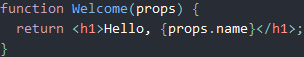
\includegraphics[scale=0.5]{react_functional_component}
	\label{fig:reactfunctionalcomponent}
\end{figure}

Class components are the heavy lifters in the React framework and typically make up the majority of the components implemented. The class components enable the developer to encapsulate the functionality of a piece of the web application to ensure that it is reusable. Likewise, utilizing class components keeps all of the necessary data associated with the markup being rendered. This structure ensures that any callbacks such as \texttt{onClick} can be swapped out since they can reference the properties of the encapsulating class. Click handlers can by dynamically assigned depending on the application's current context. This flexibility enables the developer to write generic components which can be reused and repurposed.

\begin{figure}[h]
	\centering
	\caption{React Functional Component}
	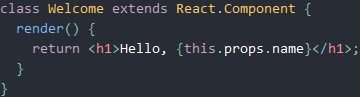
\includegraphics[scale=0.5]{react_class_component}
	\label{fig:reactclasscomponent}
\end{figure}

\printbibliography[title={References}]

\end{document}
